\begin{figure}[H]
  \centering
  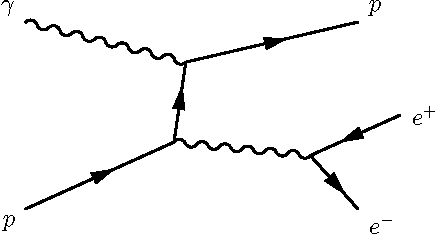
\includegraphics{feynmp/BH_pg.pdf}
\end{figure}

\begin{equation}
  P_\gamma + P_p = P_{p'} + P_{e^{+}} + P_{e^{-}}
\end{equation}
Squaring both sides, and noting that in the center-of-mass frame the outgoing particles are produced at rest, we get
\begin{equation}
  (P_\gamma + P_p)^2 = (m_p + 2m_e)^2.
\end{equation}
\begin{equation}
  (P_\gamma + P_p)^2 = P_\gamma^2 + P_p^2 + P_\gamma P_p = 0 + m_p^2 + 2 P_\gamma \cdot P_p
\end{equation}

Since the proton is ultra-relativistic,
\begin{equation}
  P_\gamma =  \begin{pmatrix} E_\gamma & -E_\gamma & 0 & 0 \end{pmatrix}
  \quad \text{and} \quad
  P_p \approx \begin{pmatrix} E_p      & E_p       & 0 & 0 \end{pmatrix}.
\end{equation}
\begin{equation}
  \therefore P_\gamma \cdot P_p = 2 E_p E_\gamma,
\end{equation}
and
\begin{equation}
  m_p^2 + 4 E_p E_\gamma = m_p^2 + 4 m_e m_p + 4 m_e^2
\end{equation}
\begin{equation}
  \boxed{ E_p = \frac{m_e m_p + m_e^2}{E_\gamma} }
\end{equation}

$m_e = 0.511\MeV$, $m_p = 938\MeV$. The temperature of the CMB is $2.726$~K which corresponds to $E_\gamma = 0.235$~meV. Substituting, we get
\begin{equation}
  E_p = \frac{0.511\times 938 + 0.511^2}{0.235} \times \frac{10^{12}}{10^{-3}} \eV
      = \boxed{ 2.04\times 10^{18} \eV }
\end{equation}

